\documentclass[conference]{IEEEtran}
\IEEEoverridecommandlockouts
% The preceding line is only needed to identify funding in the first footnote. If that is unneeded, please comment it out.
\usepackage{cite}
\usepackage{amsmath,amssymb,amsfonts}
\usepackage{algorithmic}
\usepackage{graphicx}
\usepackage{textcomp}
\usepackage{xcolor}
\usepackage{tabularx,booktabs}
\usepackage[utf8]{vietnam}
\def\BibTeX{{\rm B\kern-.05em{\sc i\kern-.025em b}\kern-.08em
    T\kern-.1667em\lower.7ex\hbox{E}\kern-.125emX}}
\begin{document}

\title{Video Understanding : A review of action detection-recognition dataset}

\author{\IEEEauthorblockN{1\textsuperscript{st} Viet Hang Duong}
\IEEEauthorblockA{\textit{Dept of Computer Science} \\
\textit{University of Information Technology}\\
Ho Chi Minh City, Viet Nam \\
hangdv@uit.edu.vn}
\and
\IEEEauthorblockN{2\textsuperscript{nd} Duc Manh Nguyen Dang}
\IEEEauthorblockA{\textit{Dept of Computer Science} \\
\textit{University of Information Technology}\\
Ho Chi Minh City, Viet Nam \\
22520847@gm.uit.edu.vn}
\and
\IEEEauthorblockN{3\textsuperscript{rd} Ngoc Tram Phan Huynh}
\IEEEauthorblockA{\textit{Dept of Computer Science} \\
\textit{University of Information Technology}\\
Ho Chi Minh City, Viet Nam \\
22521500@uit.edu.vn}
}

\maketitle

\begin{abstract}
In this article, we provide a summary and an overview of the datasets used in the task of action detection/recognition. The datasets will be presented in the order of their publication time. For each dataset, we sequentially present four aspects: the context of its creation, data distribution, explanations of annotations, and data collection methods. \\
\end{abstract}

\begin{IEEEkeywords}
Dataset Overview 
\end{IEEEkeywords}

\section{Introduction}
In video understanding tasks, action recognition and detection are prominent and meaningful due to their practical applications in daily life. Some notable applications include Surveillance and Security, Human-Computer Interaction, Sports Analysis, Entertainment and Gaming, among others. Although deep learning models designed to solve these problems often require significant computational resources, with the advancement of computer hardware, the deployment in real-world scenarios while meeting real-time processing speed has become more feasible over time.

Besides the requirement for significant computational resources, they also demand a large and sufficiently complex dataset. In addition to serving as training data, datasets also provide a portion of data specifically for evaluating models, thereby establishing a common benchmark for comparing different models. Over the years, new datasets have emerged, either as additions to existing datasets or as entirely new ones based on different construction perspectives. This has increased both the diversity and quantity of available data, but also inadvertently posed challenges in selecting an appropriate dataset. Evaluating whether a dataset is suitable for a given research problem is not merely a matter of its scale. Other characteristics must also be considered, such as the dataset creator's perspective, data collection methods, sample size, number of classes, level of annotation detail (spatial, temporal, sound, etc.), popularity within the research community, the baseline for comparison, and various other factors. Therefore, it is necessary to carefully examine datasets relevant to the task, gather information, evaluate, and then compare them to ultimately select the desired dataset for research purposes. This process typically consumes a significant amount of time and effort. To address this issue, in this paper, we aim to compile notable datasets in the fields of action detection and action recognition, listing them chronologically while providing concise necessary information regarding:

\begin{itemize}
	\item \textit{Context and construction perspective of the dataset}: Since the datasets are presented chronologically, this section clarifies the information regarding the background and the authors' perspectives on the shortcomings or the necessary additions to older datasets.
	\item \textit{Dataset distribution}: Information about the dataset, such as the number of data samples, the number of classes, the train-validation splits, and any other available details.
	\item \textit{Annotations}: Explanation of the annotations provided in the dataset.
	\item \textit{Data collection methods}: We summarize the data collection process employed by the respective author groups on that dataset. This allows for a more objective assessment of the dataset's reliability and quality based on the researcher's perspective.
\end{itemize}

In section II, we will provide a brief overview of the history and context of the field of artificial intelligence research from its inception to the emergence of CNN models and their dominance from image task to video task. Having a general understanding of the history and context will help readers understand why datasets have their limitations and continue to evolve over the years.

In section III, we will list the datasets in the order of their publication time (measured from the time the accompanying paper is published). Each dataset will include four pieces of information presented in the following order: "Context and Construction Perspective of the Dataset," "Annotations," "Dataset Distribution," and "Data Collection Methods." If some information is not provided by the authors in the original paper, it will be left blank or omitted. Additionally, if the authors provide any additional information included in the dataset, we will allocate a separate section below to describe it. The list of datasets, along with a brief overview of their publication dates and the mentioned data quantities, can be found in Fig1..

\section{Overview of History}

In the mid-1940s to 1950s, scientists from various fields posed the question of creating an artificial brain, leading to the establishment of the field of Artificial Intelligence (AI) as an academic discipline at the Dartmouth Summer Research Project on Artificial Intelligence in 1956. Since then, numerous studies have been conducted to harness the computational power of computers in addressing problems related to human-level cognition. While notable successes have been achieved, such as Deep Blue defeating reigning world chess champion Garry Kasparov on May 11, 1997, and a team from Carnegie Mellon University winning the DARPA Grand Challenge in 2007 with a self-navigating vehicle covering 55 miles in an urban environment while adhering to traffic safety measures, these accomplishments were primarily based on the application of advanced techniques and the remarkable progress in computer power, rather than revolutionary models. The field of AI has also faced challenges, experiencing two periods of stagnation known as "AI winters": one from 1974 to 1980 and another from 1987 to 1993. During these periods, funding was reduced due to unmet research expectations and limited economic benefits from commercializing AI products. It was not until the era of big data and significant advancements in computer hardware that AI gained increased attention and popularity within the research community. AI competitions began to be organized, particularly in computer vision, attracting numerous research groups. In 2010, the ImageNet Large Scale Visual Recognition Challenge (ILSVRC) \cite{ILSVRC} was initiated, aiming to build upon the success of the PASCAL VOC challenge \cite{PASCALVOC} by evaluating model performance in image recognition tasks.

ILSVRC, upon its initial launch, garnered significant attention and credibility within the research community due to its unprecedented scale of data: 1.2 million training images and 1,000 object classes. It attracted participation from top researchers in the field and further solidified its reputation.

\begin{figure} [h]
	\centering
	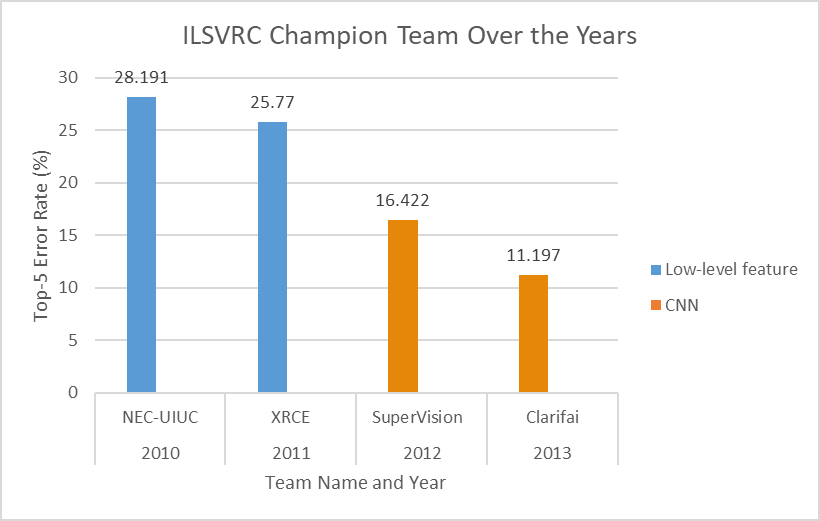
\includegraphics[width=1.\linewidth]{fig_info/fig1/ILSVRCChampionTeamOvertheYears}
	\caption{ILSVRC champion team over years on classification task}
	\label{fig:ilsvrcchampionteamovertheyears}
\end{figure}

Go back to 1998 when LeNet \cite{LeNet}, the first CNN model, was introduced. At that time, CNN was just one of many research directions and had not received much attention. It wasn't until 2012 when the SuperVison team, led by researchers at the University of Toronto, proposed a CNN model called AlexNet and convincingly won the ILSVRC2012 in image classification with a top-5 error rate of only 16.422\% (Fig \ref{fig:ilsvrcchampionteamovertheyears}). They completely outperformed other competitors at that time, paving the way for the era of CNN and the dawn of Deep Learning. Since then, winning solutions in subsequent years of ILSVRC have consistently utilized CNN. Over time, there has been an increasing number of research studies applying CNN models to various tasks. Through experimentation, CNN has proven to be effective not only in image classification but also in localization, segmentation, and even beyond computer vision, extending to other fields such as speech processing and natural language processing. CNN has shown great potential in developing solutions for previously challenging problems that were not adequately addressed. One such problem is action recognition, which is a highly significant task with practical applications. CNN has opened up possibilities for developing solutions to previously unresolved problems, and action recognition is just one of them, receiving considerable attention and practical implications.

The problem of Action Recognition existed before the rise of CNN. Solutions for action recognition during this period often involved feature extraction using various methods to obtain a feature vector from the data, followed by a classifier, typically a Support Vector Machine (SVM). The datasets used were also limited, as shown in Table \ref{config}, which lists prominent datasets from before 2012. It can be observed that in terms of scale (number of classes, number of video clips), the datasets were still quite limited.

\begin{table}[!htbp]
	\centering
	\caption{Action recognition dataset}
	\begin{tabular}{c|c c c c}
		\toprule
		Name & Year & NumClass & Clip/Class & Ref \\
		\midrule
		KTH & 2004 & 6 & 100 & \cite{KTH} \\
		Weizmann & 2005 & 9 & 9 & \cite{Weizmann} \\
		IXMAS & 2007 & 11 & 33 & \cite{IXMAS} \\
		Hollywood & 2008 & 8 & 30-129 & \cite{HollyWood} \\
		UCF Sports & 2008 & 9 & 14-35 & \cite{UCFSports} \\
		Hollywood2 & 2009 & 12 & 61-278 & \cite{Hollywood2} \\
		UCF YouTube & 2009 & 11 & 100 & \cite{UCFYouTube} \\
		Olympic & 2010 & 16 & 50 & \cite{Olympic} \\
		HMDB51 & 2011 & 51 & $\geq$ 100 & \cite{HMDB51} \\
		UCF101 & 2012 & 101 & & \cite{UCF101} \\
		\bottomrule
	\end{tabular}%
	\label{config}
\end{table}%

The CNN model, with its numerous parameters, is prone to overfitting, especially when dealing with small amounts of data. During the explosion of CNN, research groups faced many challenges due to data scarcity. Methods like data augmentation were effective solutions, but it was still necessary to supplement larger and more complex datasets to meet the growing demand for data in CNN models. This would establish a solid foundation for future research. Realizing this need, research groups from all over the AI research community have continuously improved and published increasingly refined datasets. These datasets play a crucial role as a common benchmark for comparing different models.


\bibliographystyle{ieeetr}
\bibliography{references.bib}

\end{document}
